\section{Questions}
\begin{enumerate}
\item Why do we use the complex conjugate in the inner product? I.e.
\begin{align*}
  \vec{u} \cdot \vec{v} &:= \sum_i u_i \bar{v}_i \\
  f \cdot g &:= \int f(x) \bar{g}(x) \dx
\end{align*}
\end{enumerate}



\section{Finite-dimensional vector spaces review}
\begin{enumerate}
\item What does it mean to ``project a vector into a different coordinate space?''? A simple example is the
  vector $v = \cvecc{1}{2}$. ``Projecting'' it onto the x-axis yields $\cvecc{1}{0}$, and projecting it onto the y-axis
  yields $\cvecc{0}{2}$. So, projecting here means what it sounds like: the 2D vector is collapsed onto a 1D axis,
  and we lose information about where the vector was in that other dimension.
\item What does this have to do with inner products? The inner product between vectors $a$ and $b$ is
\begin{align*}
  a \cdot b = |a| ~ |b|\cos\theta.
\end{align*}
Thus it is the area of a rectangle with one side equal to the length of the original vector and the other side
equal to the length of the projection (and it makes no difference which vector we consider to be projected).
\item Therefore, the projection of $a$ onto $b$ is
\begin{align*}
  a \cdot b
\end{align*}


  The projection onto the x-axis is computed as the inner
  product between the original vector $v$ and the x-axis basis vector $\hat{x}$:
\begin{align*}
  v \cdot \hat{x} = \cvecc{1}{2} \cdot \cvecc{1}{0} = \sum_i v_i \hat{x}_i
\end{align*}

\end{enumerate}

\section{Complex exponentials review}
\begin{enumerate}
\item $e^{xi}$ is a point on the unit circle.
\item $e^{2\pi i} = 1$ i.e. one full rotation.
\item $r(t) = e^{2\pi i t}$ is a function describing a point moving on the unit circle. If $t$ is in seconds then
  this point will perform one cycle per second (1 Hz).
\item $r(t) = e^{2\pi i f t}$ is a point rotating at a frequency of $f$ Hz. (E.g. if $f = 2$ then it will get to
  the same position in half the time.)



\section{Fourier transform}

Let $g(t)$ be a non-negative 1D continuous time series. Consider the function
\begin{align*}
  g(t)e^{-2\pi i f t}.
\end{align*}
This represents ``winding'' the time series around the unit circle (the negative sign means we are winding
clockwise).

\begin{mdframed}
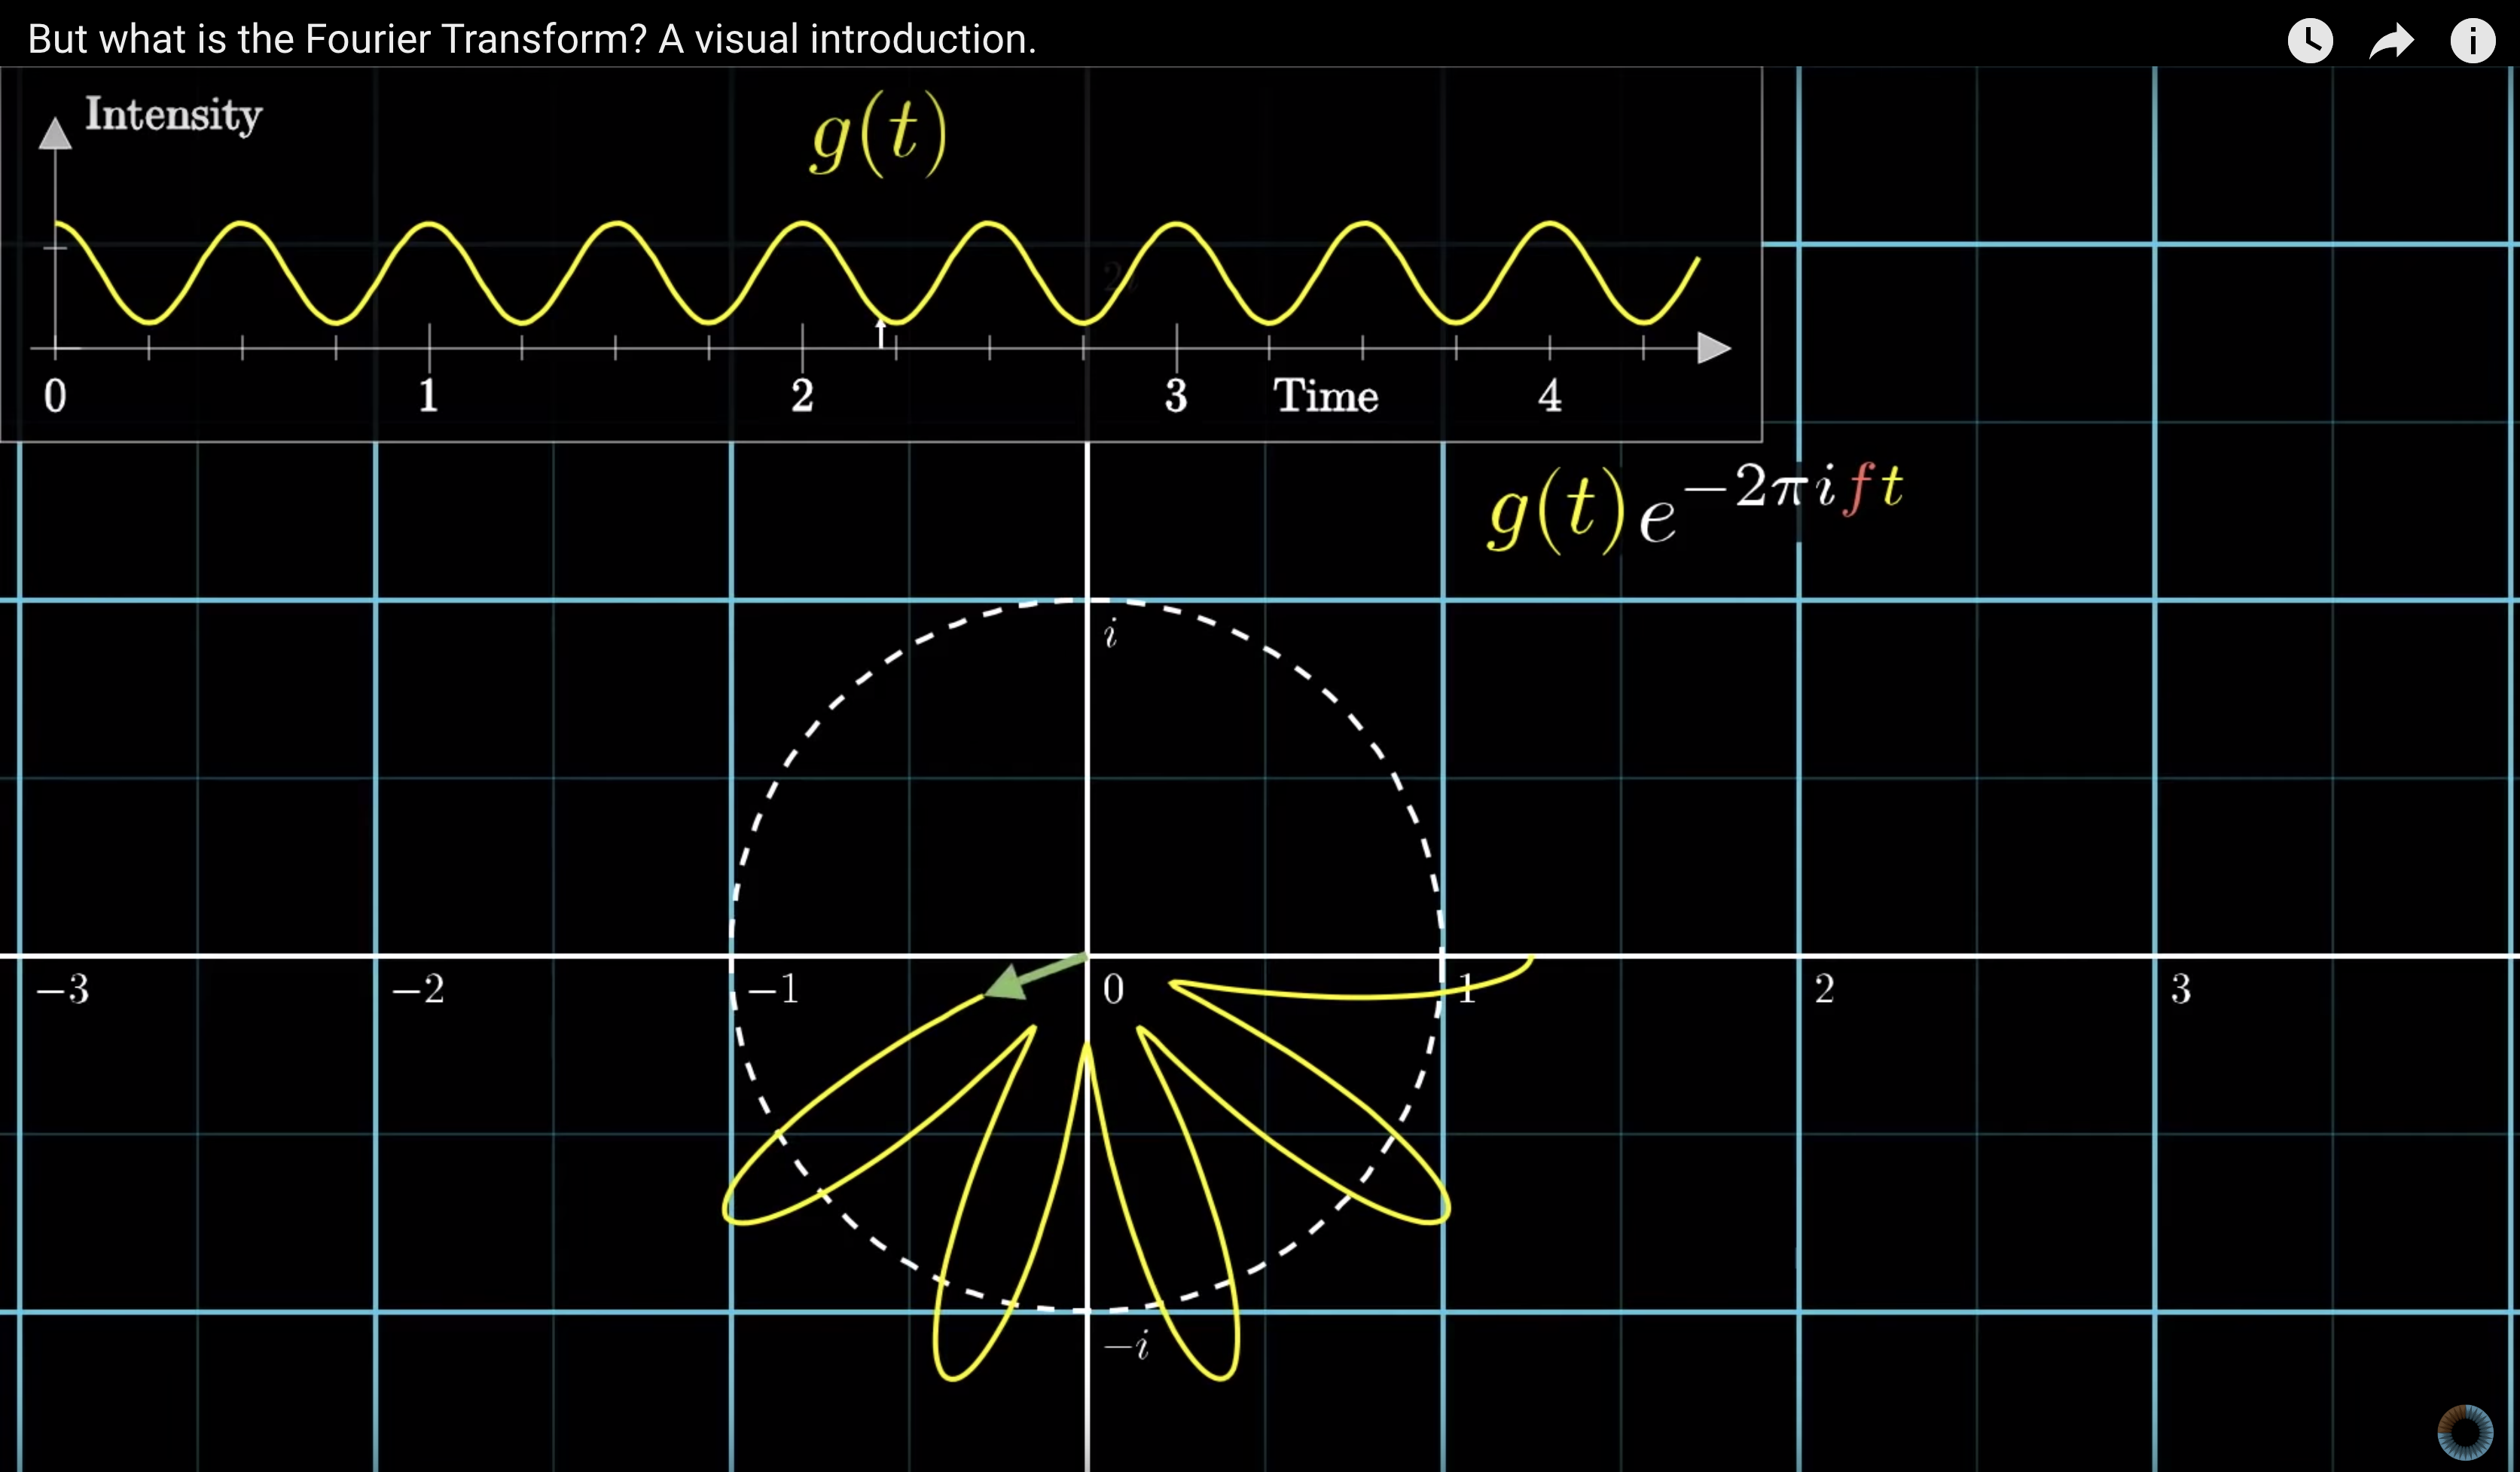
\includegraphics[width=400pt]{img/fourier--complex-exponentials-review--fourier-transform-75f4.png}
\end{mdframed}

$f$ controls the winding frequency: if $f = 1$ then the function winds around once in $2\pi$ seconds;
if $f = 2$ then the function winds around once in $\pi$ seconds.

Note that there are two frequency concepts here:
\begin{enumerate}
\item The time series $g(t)$ is composed of some mixture of sinusoids, each with a certain frequency.
\item The winding frequency $f$.

  The Fourier transform basically involves computing a ``centre of mass'' of the wound-up time series, for a
  range of $f$ values.

For most $f$ values, the centre of mass will be close to the origin.
\begin{mdframed}
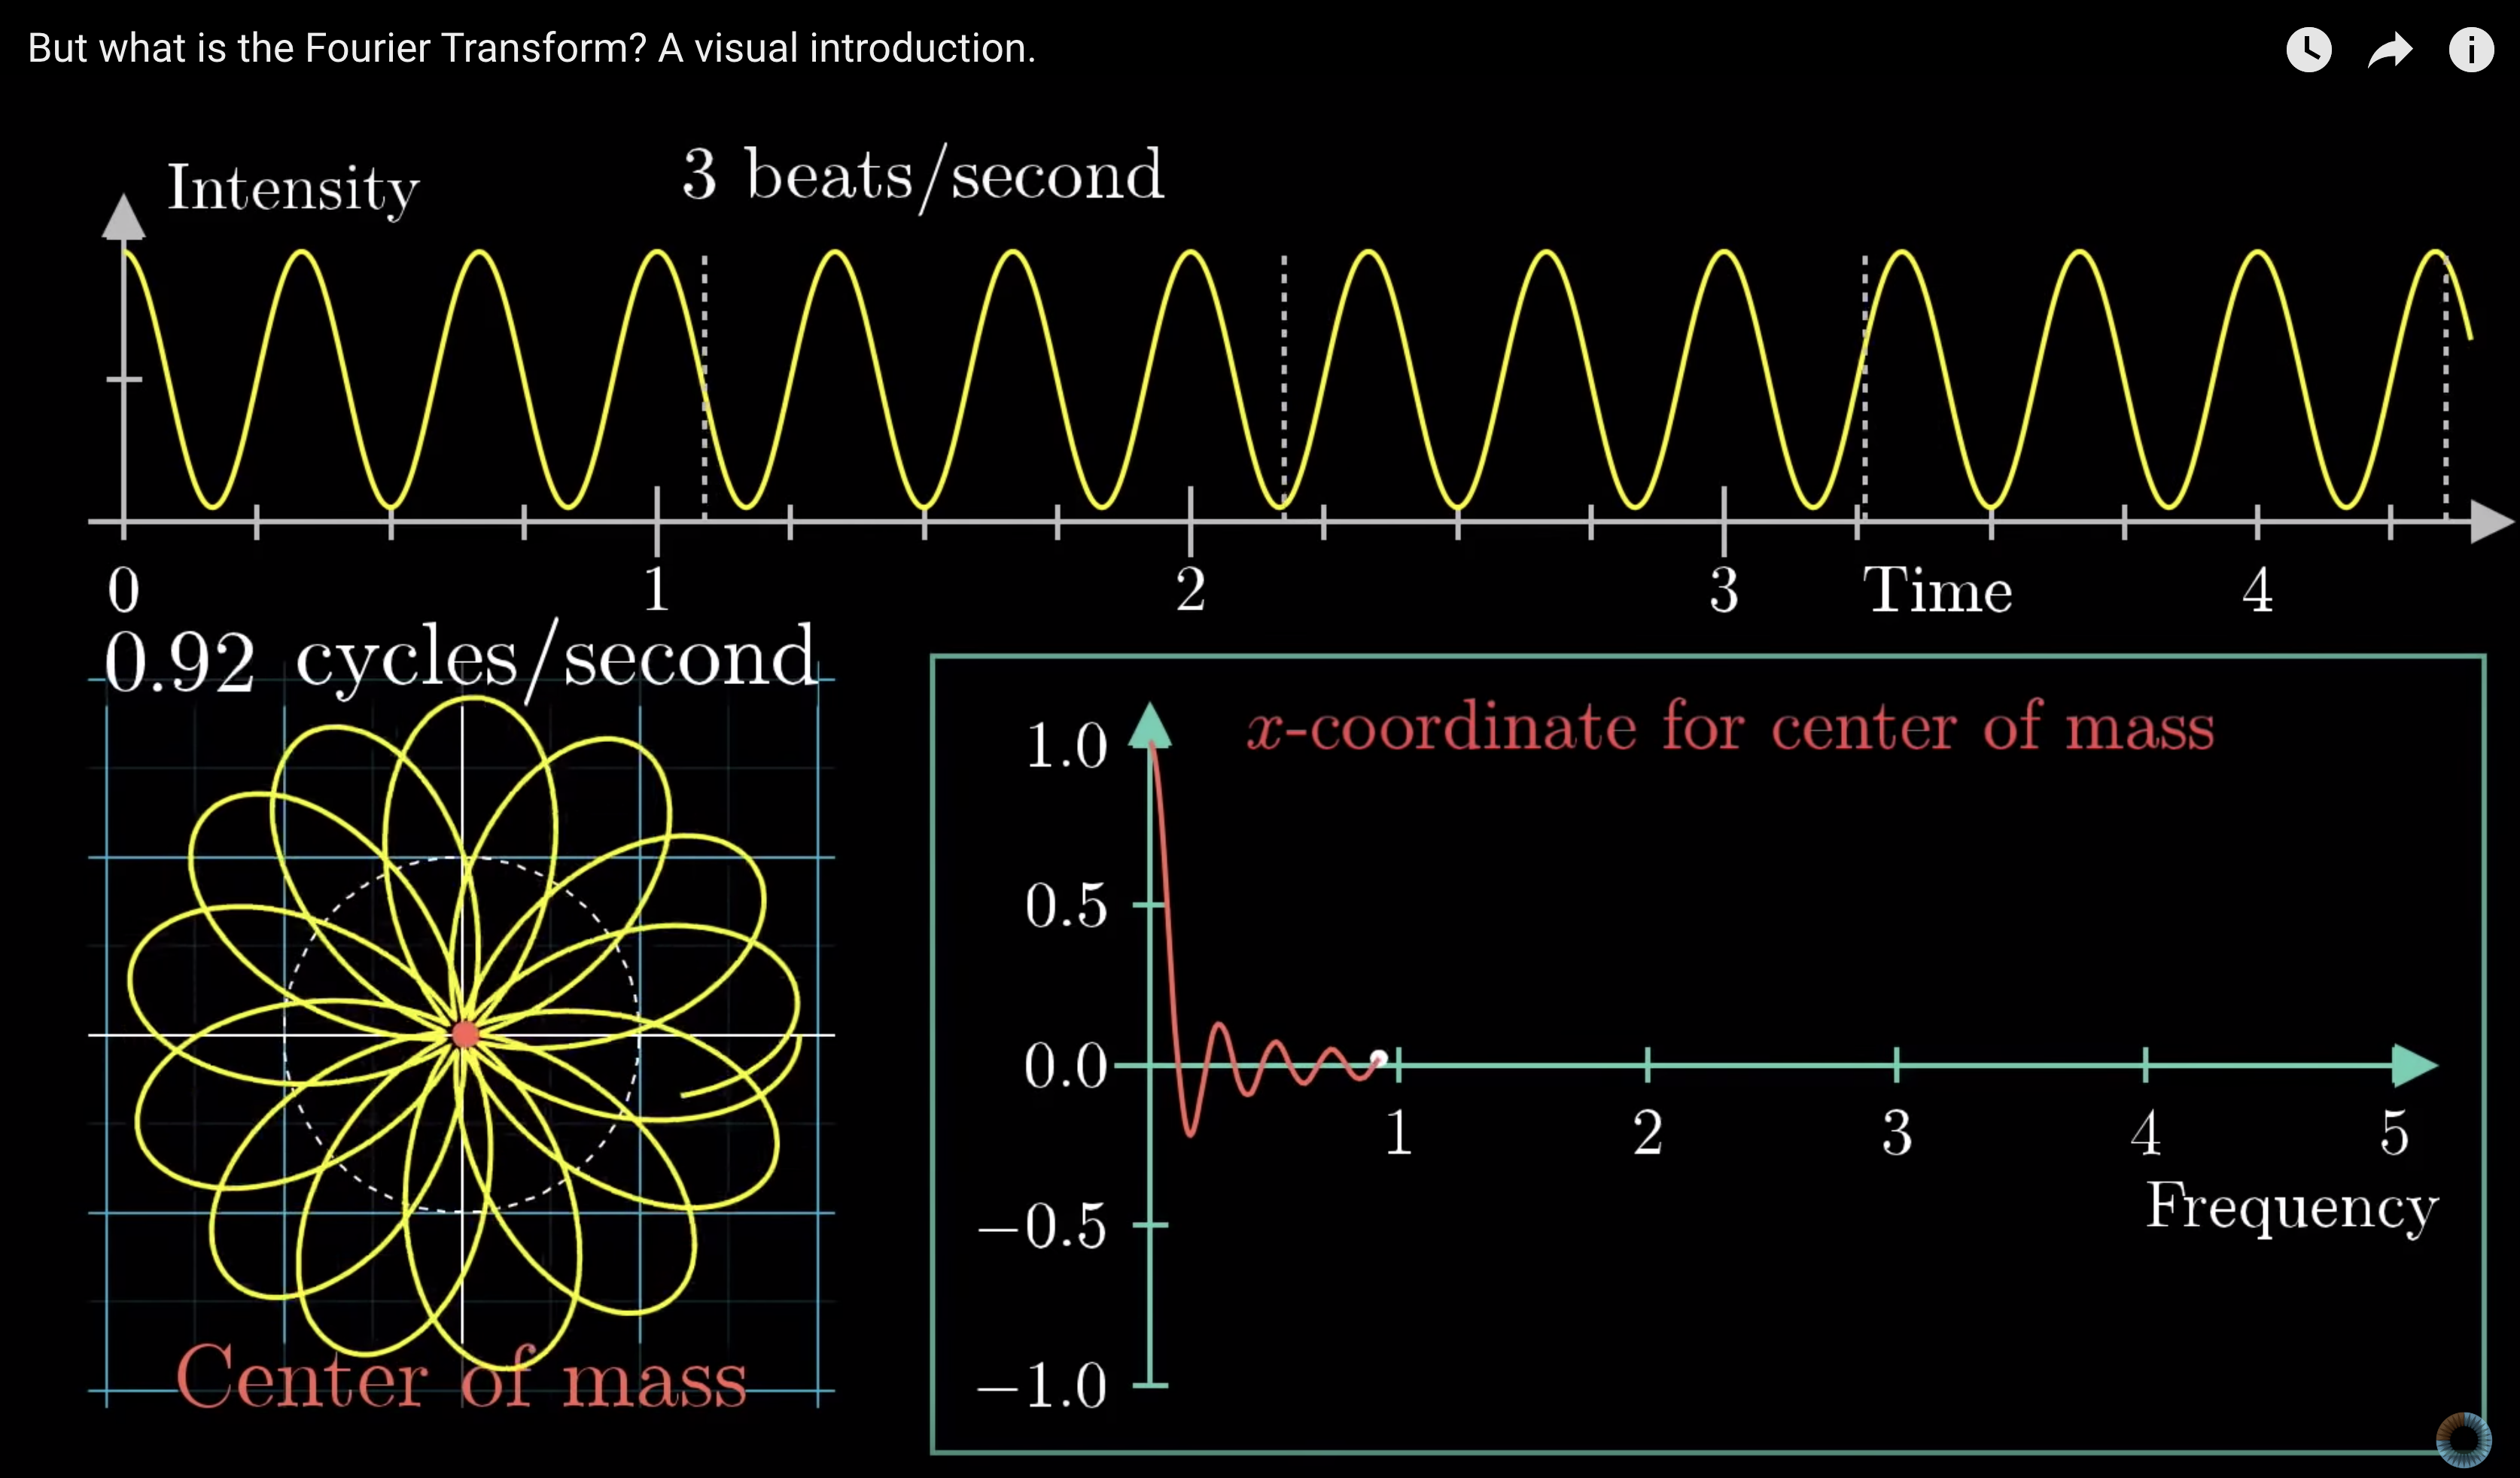
\includegraphics[width=400pt]{img/fourier--complex-exponentials-review--fourier-transform-eca1.png}
\end{mdframed}

But occasionally one will hit an $f$ value that ``resonates'' with one of the frequency components of the time
series: when this happens, the peaks of $g(t)$ will coincide, on the same side of the unit circle, and the
centre of mass will thus be far from the origin.
\begin{mdframed}
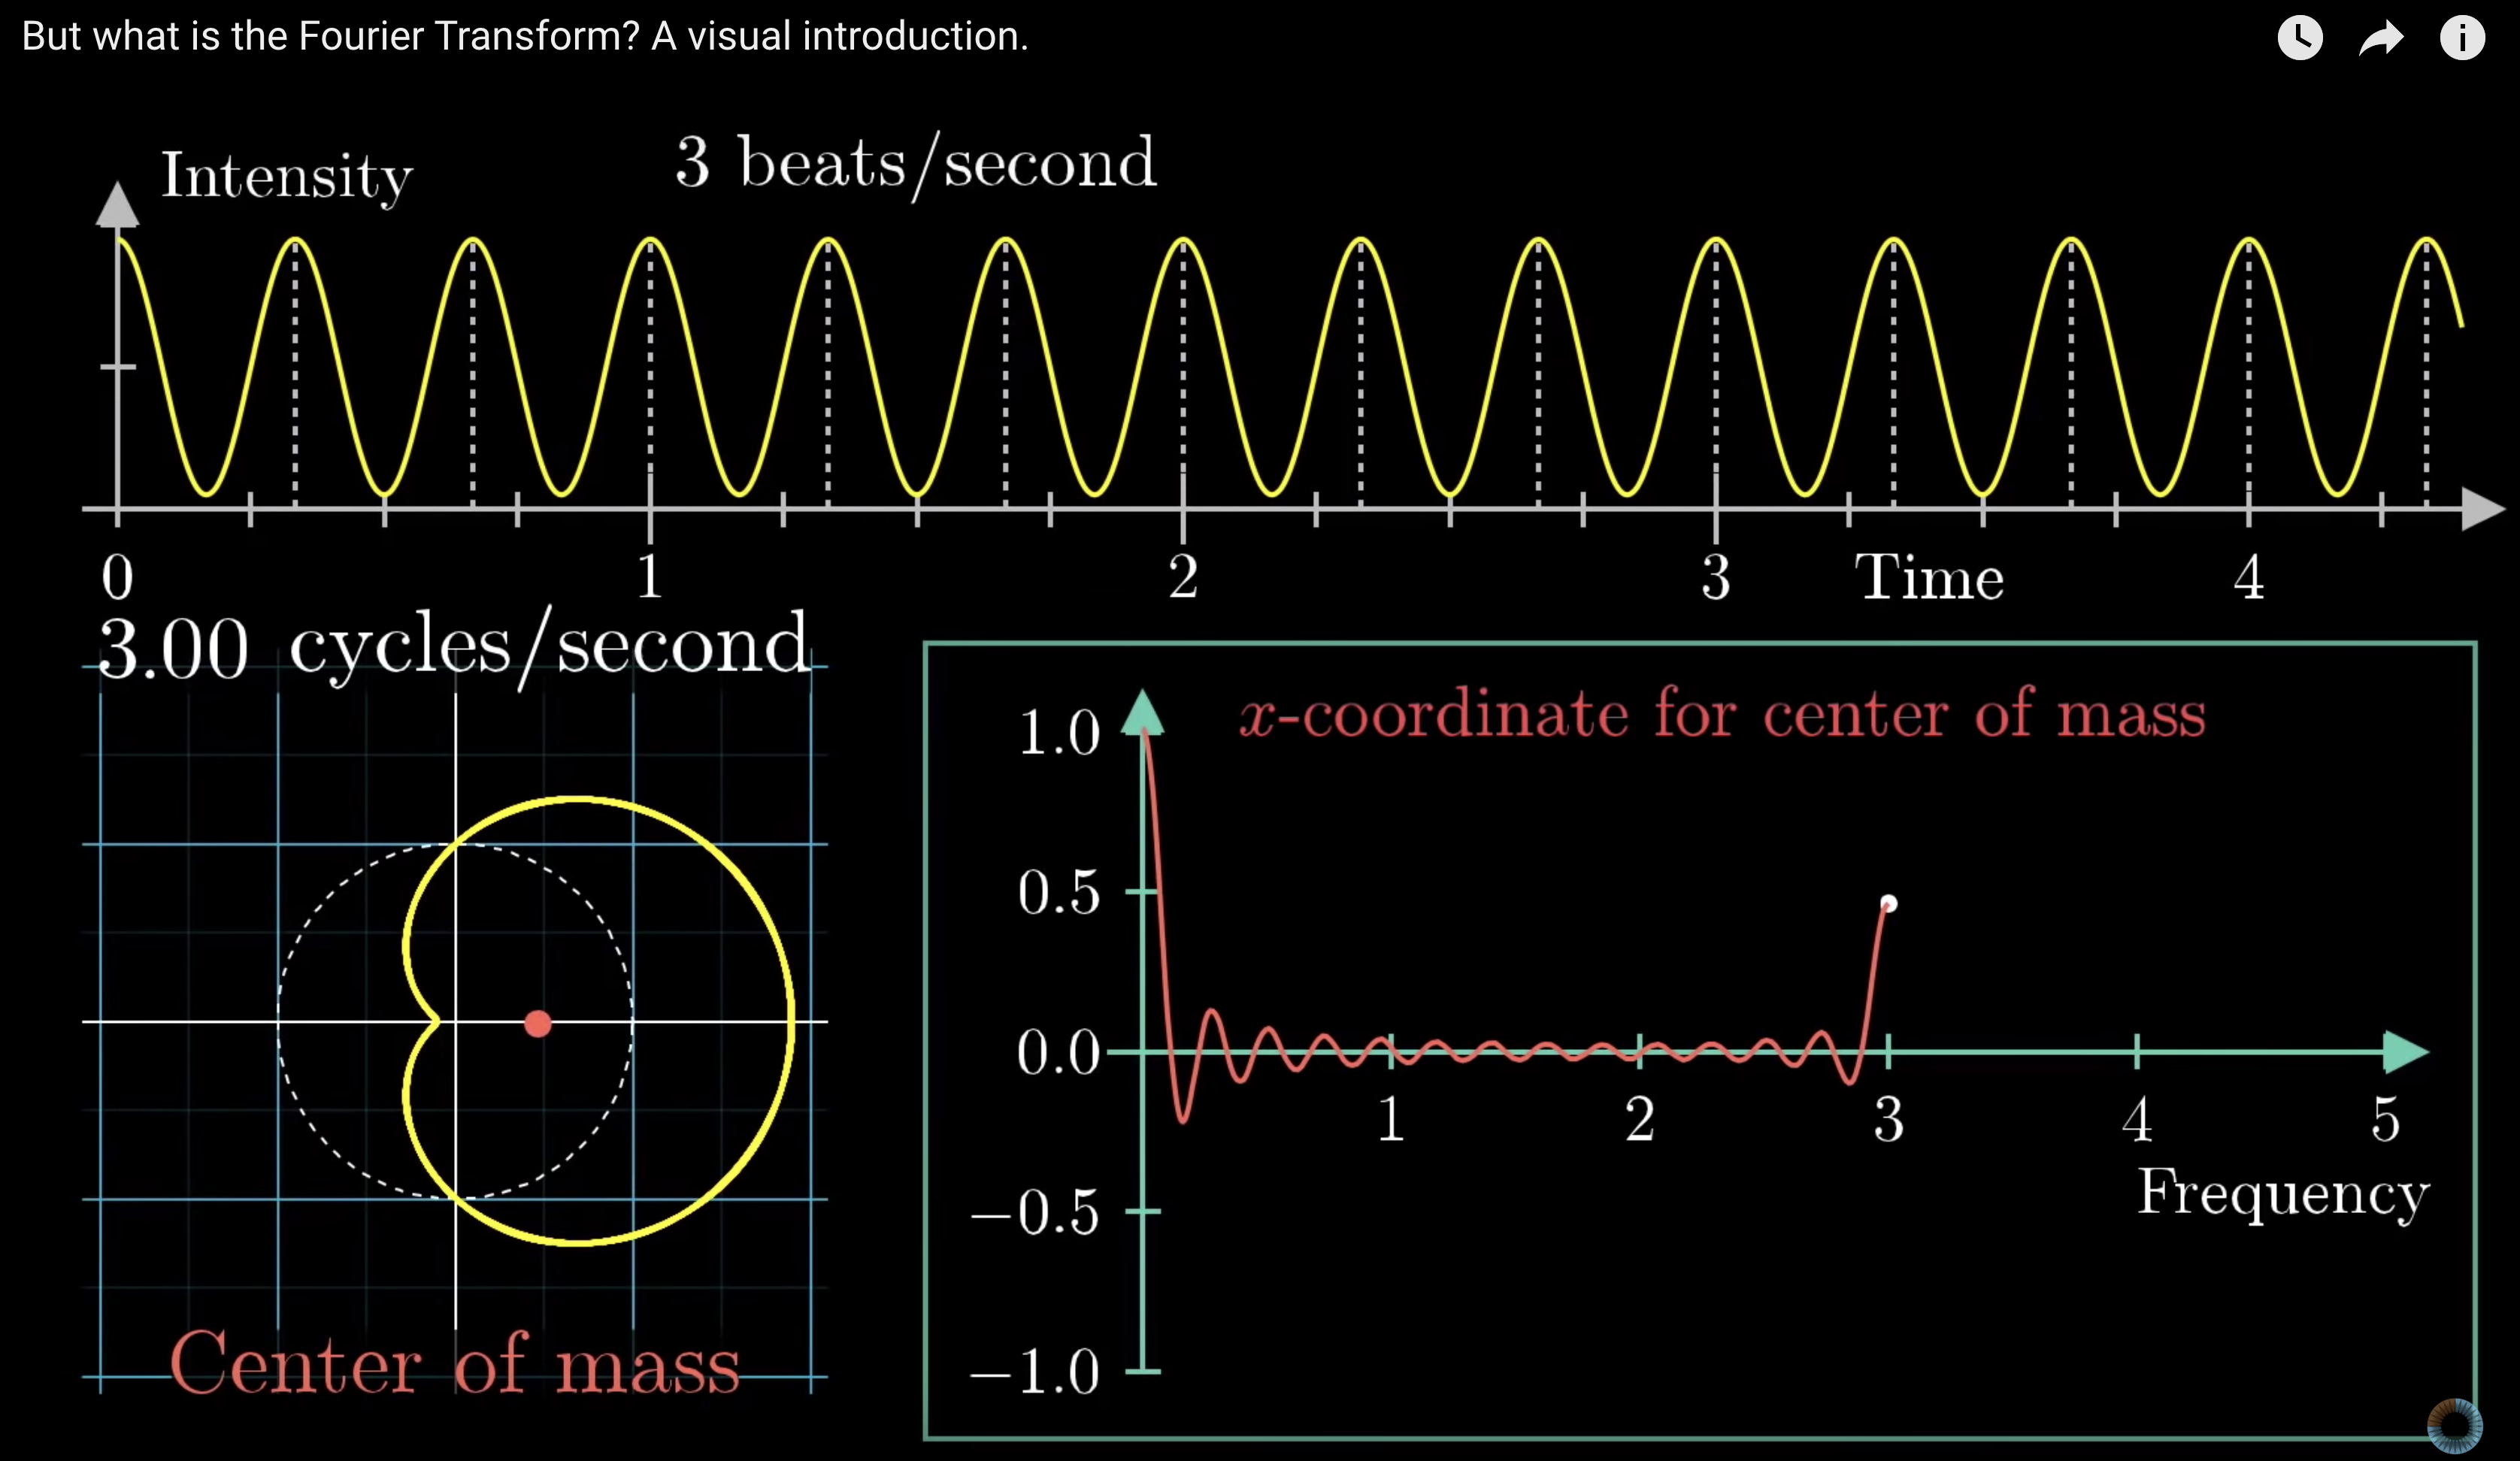
\includegraphics[width=400pt]{img/fourier--complex-exponentials-review--fourier-transform-f265.png}
\end{mdframed}
\end{enumerate}
The ``centre of mass'' of the wound-up curve is
\begin{align*}
  \frac{1}{t_2 - t_1} \int_{t_1}^{t_2} g(t)e^{-2\pi i f t} \dt.
\end{align*}
However, the Fourier transform is defined without the division, and over all time:
\begin{align*}
  \hat{g}(f) := \int_{-\infty}^{\infty} g(t)e^{-2\pi i f t} \dt.
\end{align*}
Note that $\hat{g}(f)$ is complex-valued (the centre of mass is a point in the complex plane). Often one might
just look at its real component (why not look at the modulus?).

The fact that one does not divide by the sampled time duration means that if a signal of frequency $f^*$
persists for a long time, then $\hat{g}(f^*)$ will be large: i.e. the Fourier transform emphasizes frequencies
that are present for more time.

\footnote{\url{https://www.youtube.com/watch?v=spUNpyF58BY}}
